\section{Proposed Solution}
 
The proposed solution consists in an incremental optimization approach. The core idea consists in continuously optimizing the trajectory while the UAV executes it. This however requires some additional logistics:
\begin{itemize}
    \item It is required to define at each time which part of the trajectory should be optimized
    \item It is required to have a first iteration for the trajectory optimizer
    \item It is required to have a tool that prevents the optimizer to get trapped in unfeasible local minima
\end{itemize}

\subsection{Example}

A series of figures (Fig \ref{fig:example02} - \ref{fig:example09}) will now be presented to exemplify this concept.
 \par
In most of the flight part of the trajectory is optimized while the aircraft flies.  The part of the trajectory that is executed while the optimization process runs must be fixed. This process is exemplified in Figures \ref{fig:example02} - \ref{fig:example04}.

\begin{figure}[ht!]
   \centering
   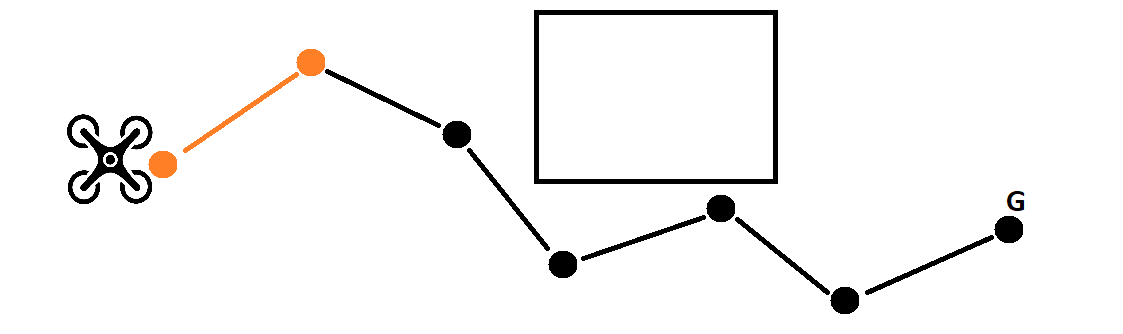
\includegraphics[width=0.6\linewidth]{Figures/03_proposed/EXAMPLE_02.png}
   \caption{Part  of  the  trajectory  fixed  (orange)  in  an  initial trajectory computed by an RRT}
   \label{fig:example02}
\end{figure}

\begin{figure}[ht!]
   \centering
   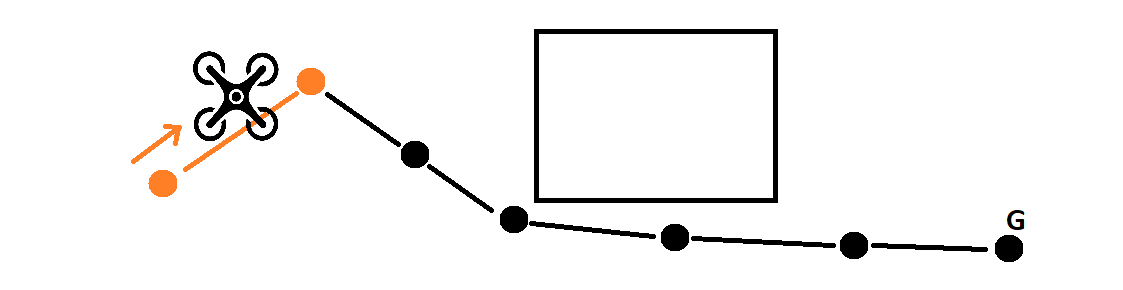
\includegraphics[width=0.6\linewidth]{Figures/03_proposed/EXAMPLE_03.png}
   \caption{Trajectory is optimized while UAV flies}
   \label{fig:example03}
\end{figure}

\begin{figure}[ht!]
   \centering
   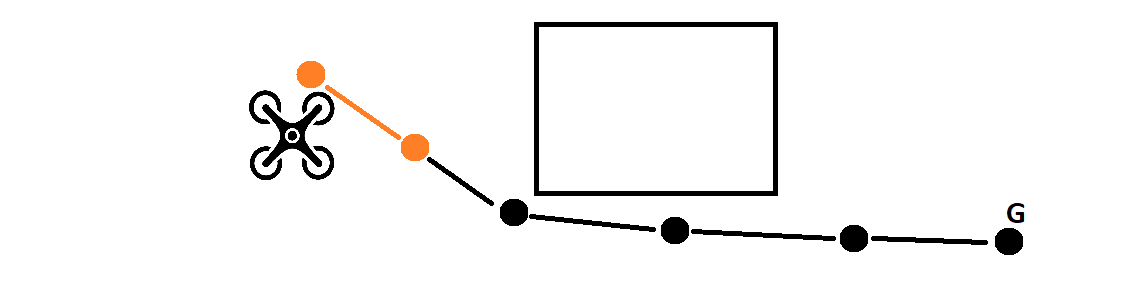
\includegraphics[width=0.6\linewidth]{Figures/03_proposed/EXAMPLE_04.png}
   \caption{New part of the trajectory is fixed and process re-starts}
   \label{fig:example04}
\end{figure}

In the case that there is some non-feasible portion in the trajectory (a part of the trajectory exceeds the maximum allowed speed or acceleration or there are collisions with obstacles) the trajectory is only optimized around the unfeasible portion (Fig \ref{fig:example05} - \ref{fig:example06}).

\begin{figure}[ht!]
   \centering
   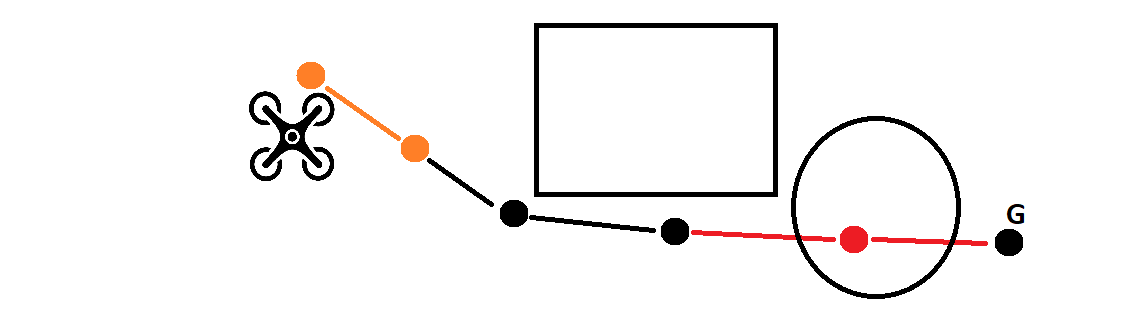
\includegraphics[width=0.6\linewidth]{Figures/03_proposed/EXAMPLE_05.png}
   \caption{Unknown obstacle detected in the trajectory}
   \label{fig:example05}
\end{figure}

\begin{figure}[ht!]
   \centering
   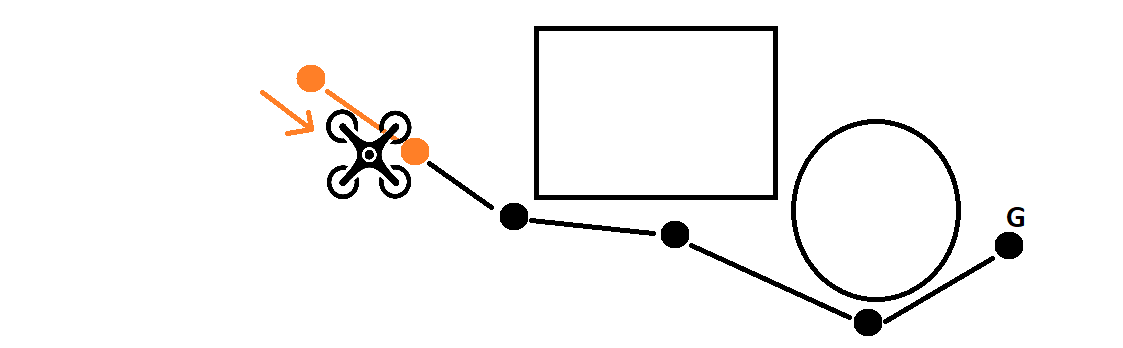
\includegraphics[width=0.6\linewidth]{Figures/03_proposed/EXAMPLE_06.png}
   \caption{Trajectory optimizer adjusts the trajectory avoiding the obstacle}
   \label{fig:example06}
\end{figure}


\par
If the optimizer can't make the trajectory feasible in a chosen, limited, number of increments (in this work it will be called the maximum number of failures ()\textit{maximumFailCount}) the RRT algorithm regrows a trajectory around the unfeasible portion (Fig \ref{fig:example08} - \ref{fig:example09}). This might happen if the trajectory falls into an unfeasible local minima.



\begin{figure}[ht!]
   \centering
   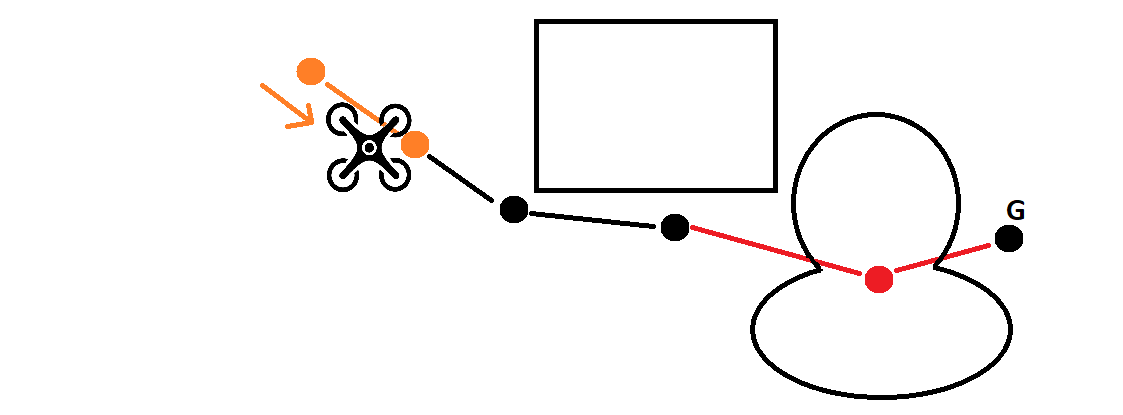
\includegraphics[width=0.6\linewidth]{Figures/03_proposed/EXAMPLE_08.png}
   \caption{Unknown complex obstacle detected in the trajectory}
   \label{fig:example08}
\end{figure}

\begin{figure}[ht!]
   \centering
   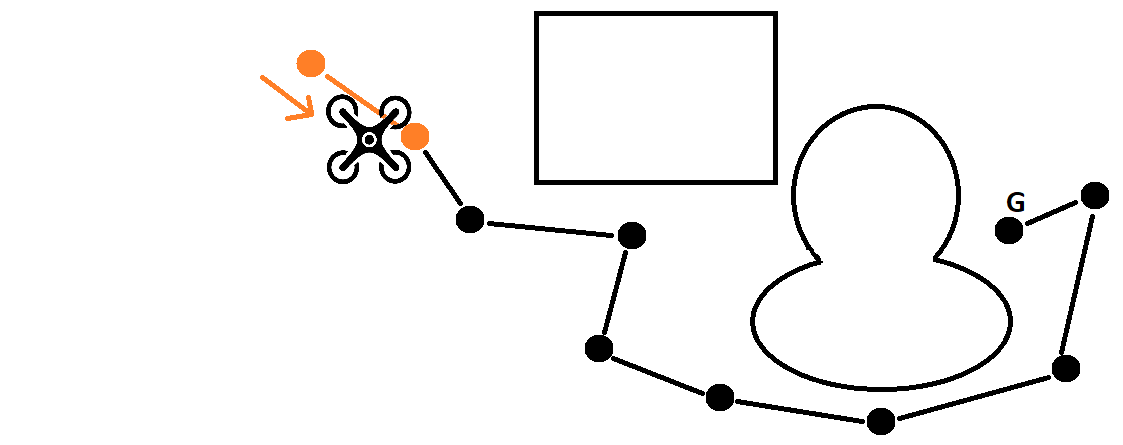
\includegraphics[width=0.6\linewidth]{Figures/03_proposed/EXAMPLE_09.png}
   \caption{The maximum number of failures is reached and a trajectory is regrown around the obstacle}
   \label{fig:example09}
\end{figure}


\par
Finally, in the case that the non-feasible part of the trajectory corresponds to a time interval that is very close to the current time $t_C$ a different approach should be taken. In this scenario the optimization increment might not be performed fast enough to avoid a collision. If this is the case the UAV enters an "emergency mode" which consists in stopping to follow the previous trajectory and recomputing the trajectory from scratch.
\par
Concerning the first iteration given to the optimizer it will be used a modified RRT. This RRT will also be used to regrow critical parts of the trajectory whenever it gets trapped in unfeasible local minima. The trajectory is computed from the UAV to the goal in the beginning of the mission and every time the robot discards the old trajectory when entering the "emergency mode".
\par
This planner requires access to two methods: one for getting the UAV position, one for getting the environment map. The behaiviour of the planner can be explainned using a state machine, represented in Fig. \ref{fig:stateMachine}.

\begin{figure}[H]
    \centering
    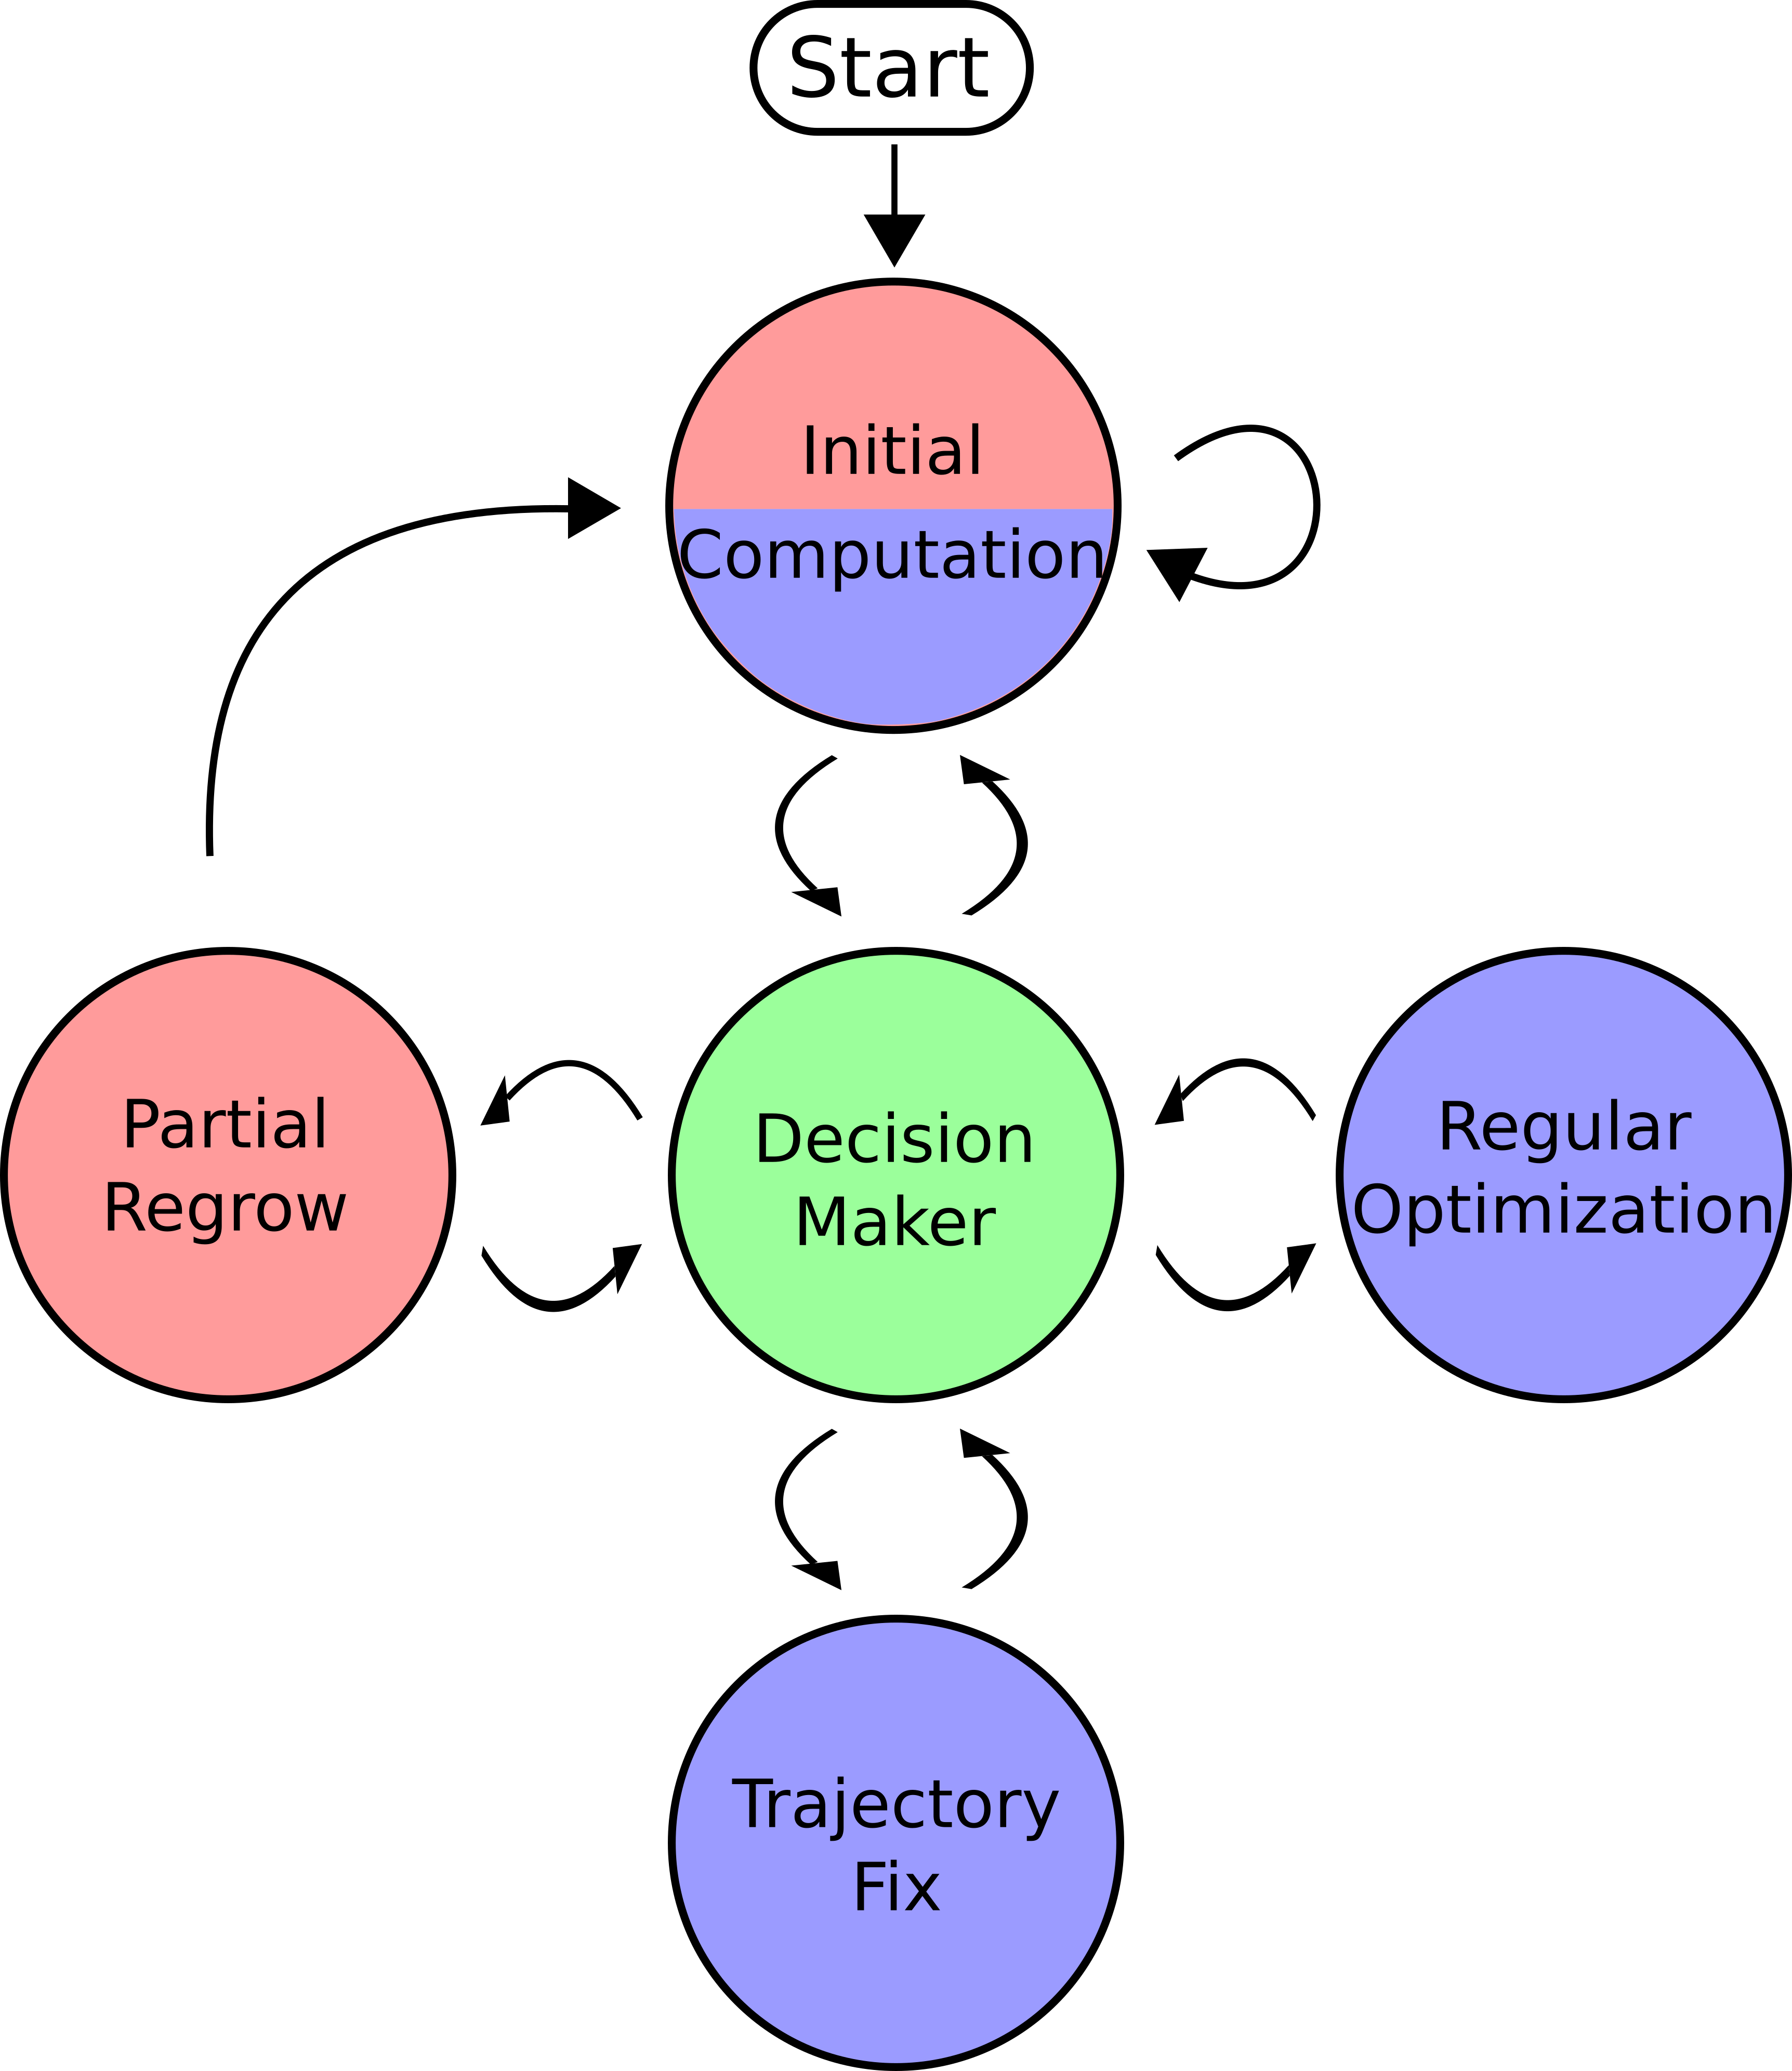
\includegraphics[width=0.6\linewidth]{Figures/06_software/stateColored.png}
    \caption{State machine describing the real-time trajectory planner. Red, blue and green states use methods from the \textbf{RRT}, \textbf{Optimizer} and \textbf{Feasibility Tester} scripts respectively.}
    \label{fig:stateMachine}
\end{figure}

\subsection{Initial Computation}

When the algorithm starts (and in some other situations) it enters the \textit{Initial Computation} state. When this state is entered the UAV position is used as the starting state and if there is a trajectory, it is discarded. Then, a trajectory is computed using an RRT. If the RRT fails to compute a trajectory in a given time (\textit{initialRRTTimeOut}) this state is re-started. If, on the other hand, the RRT can successfully compute a trajectory, a defined portion of that same trajectory is optimized for a defined time (\textit{initialOptimizationTime}). This is where the anytime capability of the algorithm is evident, the  \textit{initialOptimizationTime} parameter controls the equilibrium between computational time and trajectory quality.

\subsection{Regular Optimization}
\begin{figure}[!ht]
   \centering
   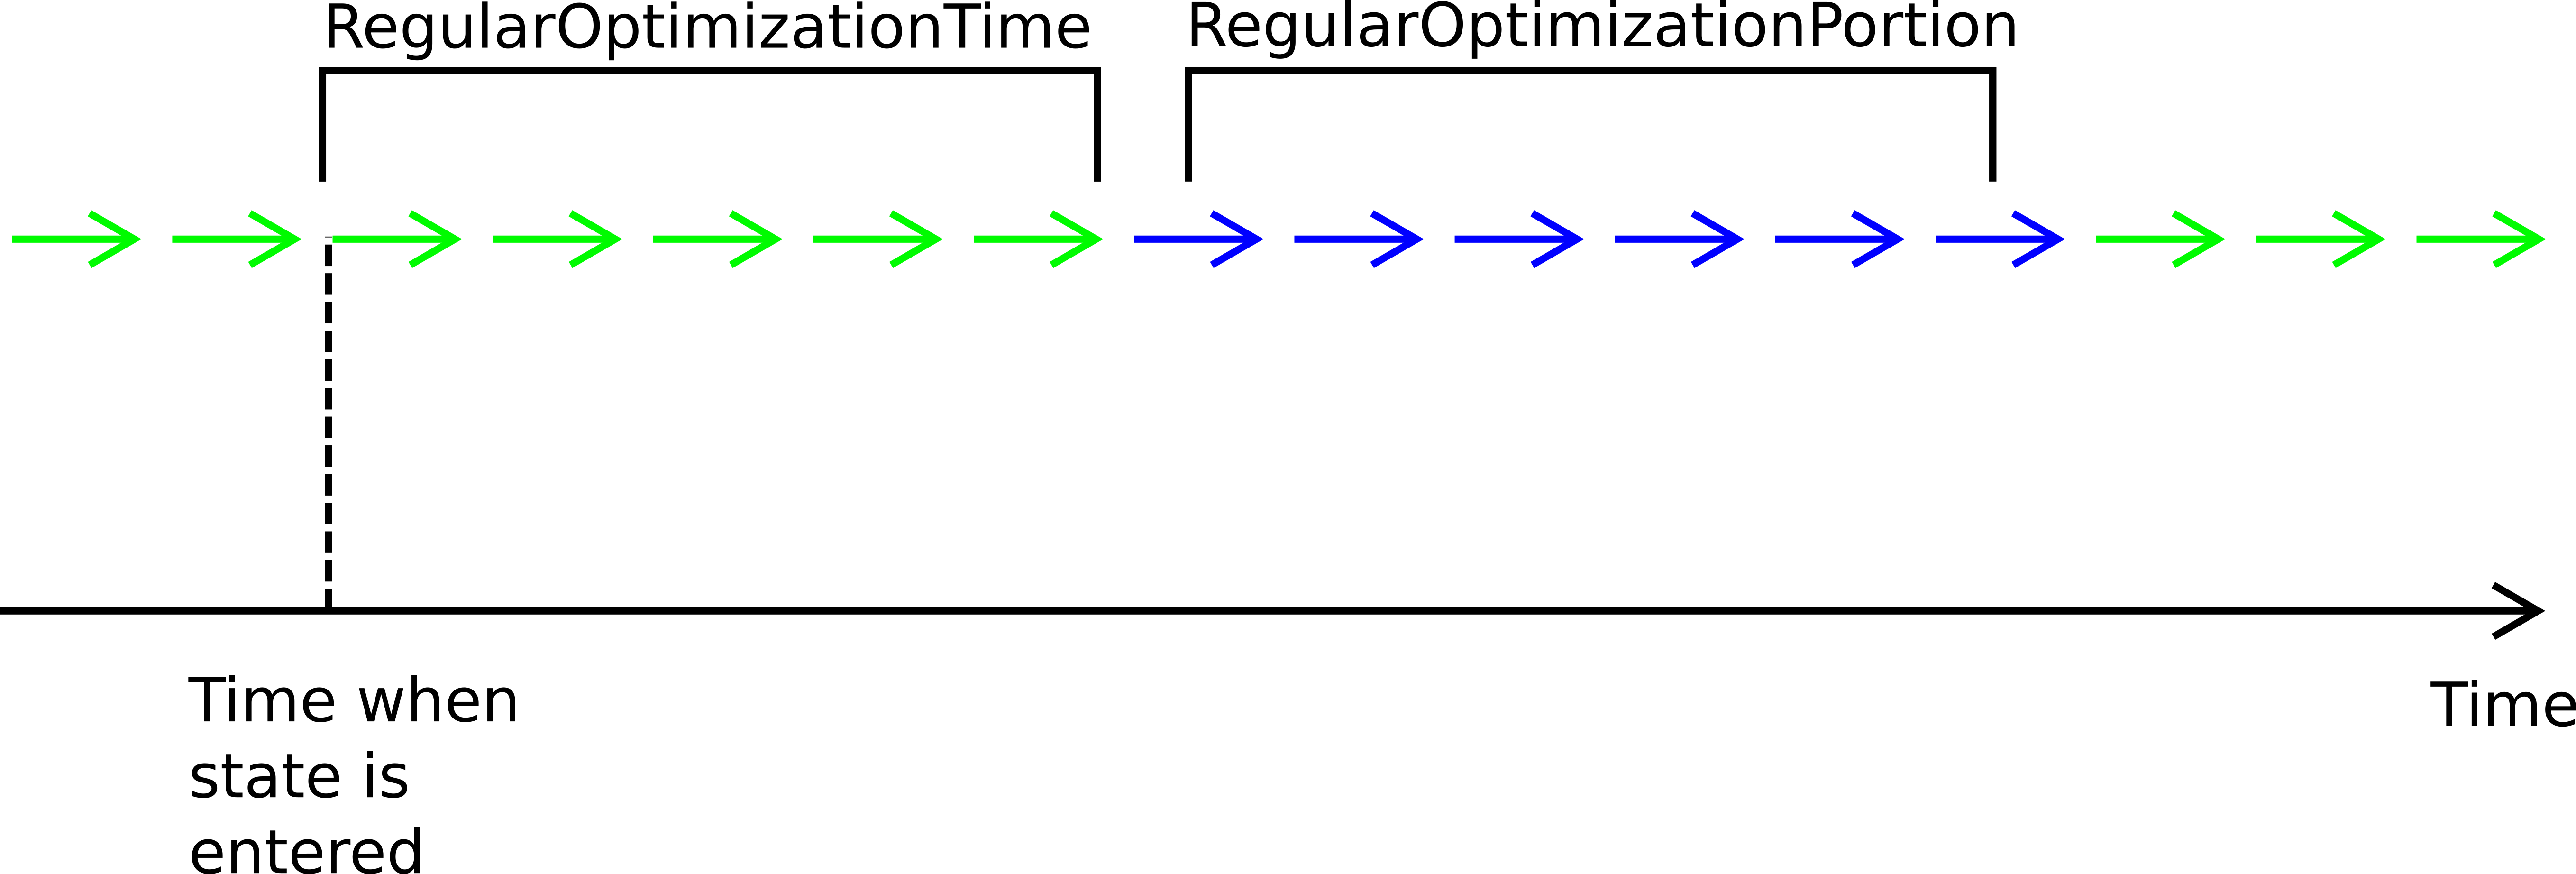
\includegraphics[width=0.9\linewidth]{Figures/06_software/regOptTime.png}
   \caption{Portion of trajectory that is optimized in the \textit{Regular Optimization} state is represented as a series of blue arrows. The first and last blue arrows are treated as a local start and a local goal (these waypoints are fixed during the optimization).}.
   \label{fig:regOptTime}
\end{figure}

In this state a portion of the trajectory ahead of the UAV is optimized for a period of time defined by the parameter \textit{regularOptimizationTime}. When this state is entered the algorithm chooses a portion of the trajectory between the point \textit{regularOptimizationTime} ahead of the current time and another point ahead defined by the parameter \textit{regularOptimizationPortion}. The portion of the trajectory which is optimized is shown in Figure \ref{fig:regOptTime}. This choice assures that when the optimization is complete and the trajectory is updated, the UAV is not executing the updated part of the trajectory.

\subsection{Trajectory Fix}
\begin{figure}[!ht]
   \centering
   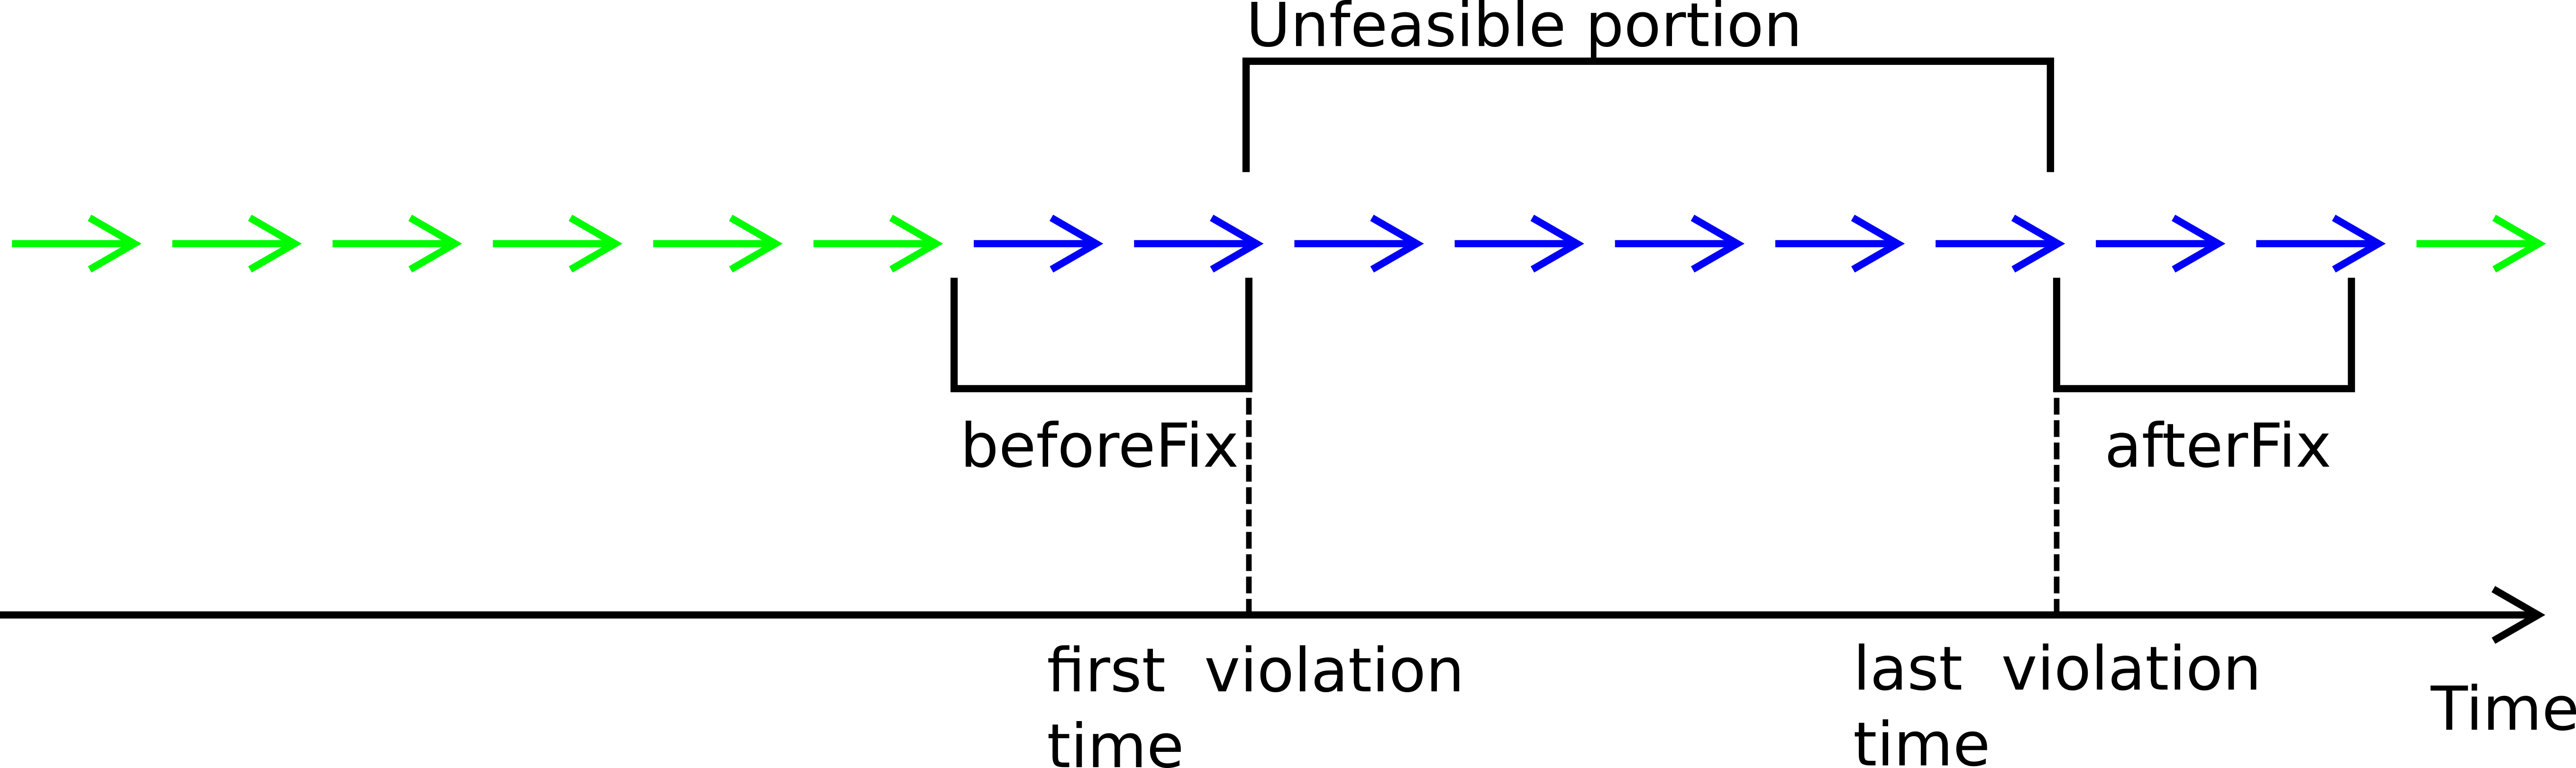
\includegraphics[width=0.9\linewidth]{Figures/06_software/fixOptTime.png}
   \caption{Portion of trajectory (blue) that is optimized in the state \textit{Trajectory Fix}. The first and last blue arrows are treated as a local start and a local goal (these way-points are fixed during the optimization.}
   \label{fig:fixOptTime}
\end{figure}

The state \textit{Trajectory Fix} is called when there is an unfeasible portion of the trajectory. It optimizes a portion of the trajectory for a certain time (\textit{trajectoryFixTime}) part of the trajectory is controlled by the parameters \textit{beforeFix} and \textit{afterFix}. The trajectory is optimized between the time of the first violation minus \textit{beforeFix} and the time of the last violation plus \textit{afterFix}. Figure \ref{fig:fixOptTime} illustrates how this portion is defined.




\subsection{Partial Regrow}
This state is called when the planner is trapped in an unfeasible local minima. Unlike the other states, where the trajectory is segmented based on time, this method separates the trajectory based on distance. It regrows the trajectory between the state that is at a distance \textit{beforeRegrow} before the first violation index until \textit{afterRegrow} after the last violation index, as shown in Figure \ref{fig:regrowDistance}. The time-out associated with this state is called \textit{regrowTimeOut} and, if it is not possible to compute a trajectory within this time, the algorithm jumps to the \textit{Initial Computation} state.

\begin{figure}[H]
   \centering
   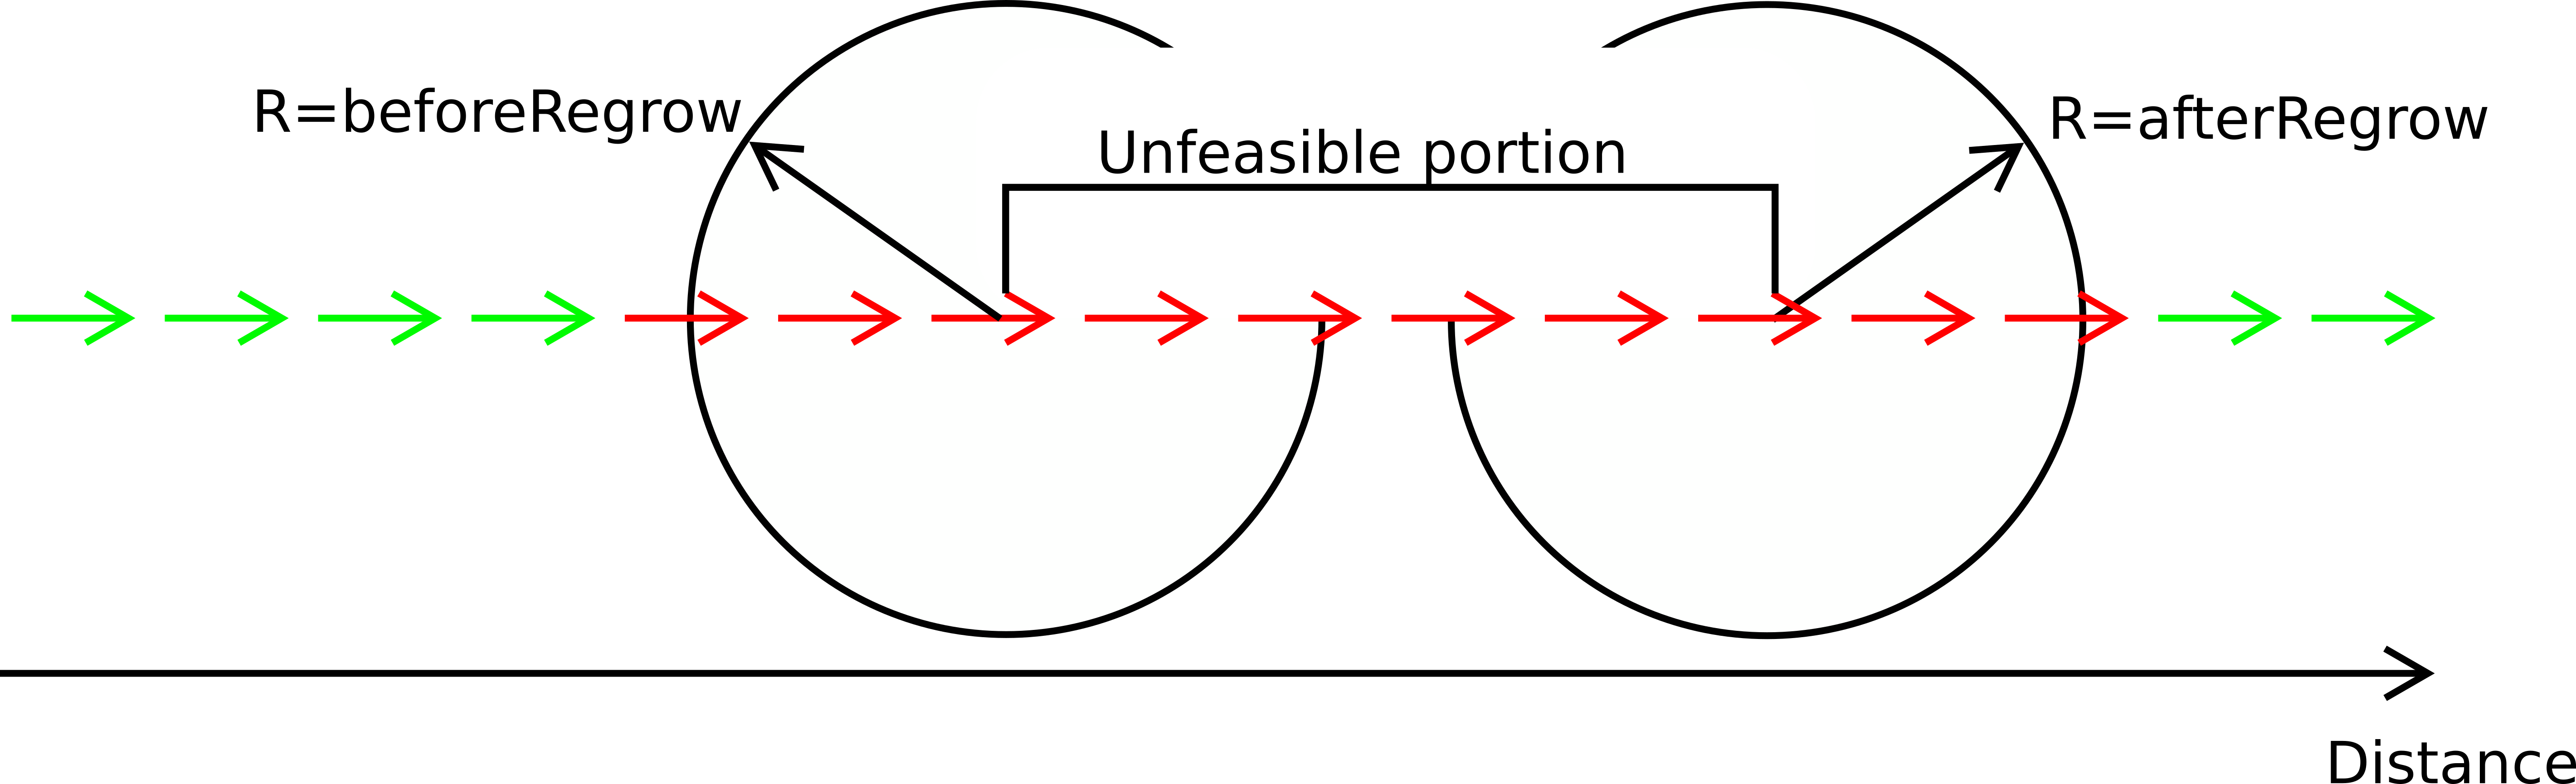
\includegraphics[width=0.9\linewidth]{Figures/06_software/regrowDistance.png}
   \caption{Portion of trajectory (red) that regrown in state \textit{Partial Regrow}. The first and last red arrows are treated as a local start and a local goal for the RRT algorithm.}
   \label{fig:regrowDistance}
\end{figure}


\subsection{Decision Maker}
The process behind the \textit{Decision Maker} defines the strategy of this algorithm. Its working principles will now be explained.
\par
This state doesn't have an associated timeout. Instead, when the algorithm enters this state it is quickly set to another state. Basically, this state is responsible for determining the future state of the algorithm. A parameter called \textit{failCount} is set to 0 after the initial computation. In this state, it is checked if there are any violations of the constraints in the trajectory (bad kinematics, maximum speed exceeded, maximum acceleration exceeded or too close to an obstacle). If there isn't any violation, then \textit{failCount} is set to 0 and the algorithm jumps to the \textit{Regular Optimization} state. If there is a failure, it is checked if the first violation time is closer than a defined \textit{criticalClearence}. If it is then the UAV is commanded to stop, \textit{failCount} is set to zero and the algorithm jumps to the \textit{Initial Computation} state. This represents an emergency stop of the UAV, to deal with critical situations. If the first violation time is after the defined \textit{criticalClearence} than the \textit{failCount} is incremented. If the \textit{failCount} reaches a defined maximum (\textit{maximumFailCount}), the \textit{failCount} is set to 0 and the algorithm jumps to the \textit{Partial Regrow} state. Otherwise the algorithm jumps to the \textit{Trajectory Fix} state.